%%%%%%%%%%%%%%%%%%%%%%%%%%%%%%%%%%%%%%%%%%%%%%%%%%%%%%%%%%%%%%%%%%%%%%%
%%%%%%%%%%%%%%%%%%%%%%%%%%%%%%%%%%%%%%%%%%%%%%%%%%%%%%%%%%%%%%%%%%%%%%% 
%%%%%%%%%%%       								 Preamble				         	                                                        %%%%%%%%%% 
%%%%%%%%%%%%%%%%%%%%%%%%%%%%%%%%%%%%%%%%%%%%%%%%%%%%%%%%%%%%%%%%%%%%%%% 
%%%%%%%%%%%%%%%%%%%%%%%%%%%%%%%%%%%%%%%%%%%%%%%%%%%%%%%%%%%%%%%%%%%%%%% 
\documentclass[10pt]{beamer}
\usepackage{setspace}
\usepackage{color}
\usepackage{amsmath,lmodern}
\usepackage{hyperref}
\usepackage{graphicx}
\usepackage{multirow}
\usepackage{tikz}
\usetikzlibrary{fit,shapes.misc}
\usepackage{pdflscape}
\usepackage{amsmath}
\usepackage{lscape}
\usepackage{multirow}
\usepackage{enumerate}
\usepackage{epstopdf}
\usepackage{pdfpages}
\usepackage{appendixnumberbeamer}
\usepackage{color,soul}
\usepackage{grffile}
\usepackage{float}
\usepackage{relsize}
\usepackage{tcolorbox}
\newcounter{nodemarkers}
\usepackage{tikz}
\newcommand{\toplinesmall}{%
  \tikz[remember picture,overlay] {%
    \draw[blue,thick] ([yshift=-1cm, xshift=.9cm]current page.north west)
             -- ([yshift=-1cm,xshift=3.6cm]current page.north west);}}
             
\newcommand{\toplinemedium}{%
  \tikz[remember picture,overlay] {%
    \draw[blue,thick] ([yshift=-1cm, xshift=.9cm]current page.north west)
             -- ([yshift=-1cm,xshift=6.2cm]current page.north west);}}
 
 \newcommand{\toplinelarge}{%
  \tikz[remember picture,overlay] {%
    \draw[blue,thick] ([yshift=-1cm, xshift=.9cm]current page.north west)
             -- ([yshift=-1cm,xshift=8.9cm]current page.north west);}}           
             
 \newcommand{\toplinexlarge}{%
  \tikz[remember picture,overlay] {%
    \draw[blue,thick] ([yshift=-1cm, xshift=.9cm]current page.north west)
             -- ([yshift=-1cm,xshift=12cm]current page.north west);}}                       
             
\setbeamertemplate{footline}
{
  \leavevmode%
  \hbox{%
  \begin{beamercolorbox}[wd=.333333\paperwidth,ht=2.25ex,dp=1ex,center]{author in head/foot}%
    \usebeamerfont{author in head/foot}{\textcolor{blue}{ECON311}}
  \end{beamercolorbox}%
  \begin{beamercolorbox}[wd=.333333\paperwidth,ht=2.25ex,dp=1ex,center]{title in head/foot}%
    \usebeamerfont{title in head/foot}{\textcolor{blue}{Winter 2026}}
  \end{beamercolorbox}%
  \begin{beamercolorbox}[wd=.333333\paperwidth,ht=2.25ex,dp=1ex,right]{date in head/foot}%
    \usebeamerfont{date in head/foot}{\textcolor{blue}{Lecture 11 \: \: \: \: \: \: \: }
    \insertframenumber{} / \inserttotalframenumber\hspace*{2ex}} 
  \end{beamercolorbox}}%
  \vskip0pt%
}
\newtheorem{proposition}[theorem]{Proposition}

\newcommand\marktopleft[1]{%
    \tikz[overlay,remember picture] 
        \node (marker-#1-a) at (-0.2,1.2ex) {};%
}
\newcommand\markbottomright[1]{%
    \tikz[overlay,remember picture] 
        \node (marker-#1-b) at (0.16,-1ex) {};%
    \tikz[overlay,remember picture,thick,inner sep=4pt]
        \node[draw,rectangle,rounded corners, blue, fit=(marker-#1-a.center) (marker-#1-b.center)] {};%
}

\setbeamertemplate{caption}{\raggedright\insertcaption\par}
\setbeamertemplate{itemize items}[ball]
\setbeamertemplate{itemize subitem}[triangle]
\setbeamertemplate{itemize subsubitem}[triangle]
\tcbset{colframe=white,colback=white,nobeforeafter}
\beamertemplatenavigationsymbolsempty
\addtobeamertemplate{frametitle}{\vspace*{0.19cm}}{\vspace*{0cm}}


%%%%%%%%%%%%%%%%%%%%%%%%%%%%%%%%%%%%%%%%%%%%%%%%%%%%%%%%%%%%%%%%%%%%%%%
%%%%%%%%%%%%%%%%%%%%%%%%%%%%%%%%%%%%%%%%%%%%%%%%%%%%%%%%%%%%%%%%%%%%%%% 
%%%%%%%%%  									    Define Title									                                       %%%%%%%%%
%%%%%%%%%%%%%%%%%%%%%%%%%%%%%%%%%%%%%%%%%%%%%%%%%%%%%%%%%%%%%%%%%%%%%%%
%%%%%%%%%%%%%%%%%%%%%%%%%%%%%%%%%%%%%%%%%%%%%%%%%%%%%%%%%%%%%%%%%%%%%%% 
\title{ECON 311} 
\author{Lecture 11: Inflation and Introduction to SR Macroeconomics}
\date{}
\AtBeginSection[]
{
 \begin{frame}<beamer>
 \tableofcontents[currentsection]
 \end{frame}
}
%%%%%%%%%%%%%%%%%%%%%%%%%%%%%%%%%%%%%%%%%%%%%%%%%%%%%%%%%%%%%%%%%%%%%%%
%%%%%%%%%%%%%%%%%%%%%%%%%%%%%%%%%%%%%%%%%%%%%%%%%%%%%%%%%%%%%%%%%%%%%%% 
%%%%%%%% 						     				Document								                                                %%%%%%%%
%%%%%%%%%%%%%%%%%%%%%%%%%%%%%%%%%%%%%%%%%%%%%%%%%%%%%%%%%%%%%%%%%%%%%%%
%%%%%%%%%%%%%%%%%%%%%%%%%%%%%%%%%%%%%%%%%%%%%%%%%%%%%%%%%%%%%%%%%%%%%%% 
\begin{document}
\setbeamercovered{transparent}

\begin{frame}
\maketitle
\end{frame}

\section{Growth Accounting}


\begin{frame}
\frametitle{\: \: \: Solow and Romer}
\toplinemedium
We combine Romer and Solow:
\begin{eqnarray*} 
Y_t=F(K_t,L_t,A_t)=A_t \: K_t^{\frac{1}{3}} \: L_{Y_t}^{\frac{2}{3}}
\end{eqnarray*}
\begin{eqnarray*}
\begin{array}{l}
L_{A_t}=\overline{l} \: \overline{L} \\[3ex]
L_{Y_t}=(1-\overline{l}) \: \overline{L} \\[3ex] 
\end{array}
\end{eqnarray*}
\begin{eqnarray*}
\begin{array}{l}
\underbrace{\frac{A_{t+1}-A_t}{A_t}}_{g_{A_t}}=\overline{z}  \: L_{A_t}
\end{array}
\end{eqnarray*}
\begin{eqnarray*}
\underbrace{\frac{K_{t+1}-K_t}{K_t}}_{g_{K_t}}=\overline{s} \: \frac{Y_t}{K_t}-\overline{d}
\end{eqnarray*}
\end{frame}

\begin{frame}
\frametitle{\: \: \: Solow and Romer}
\toplinemedium
\begin{itemize}
\item In the long-run equilibrium (BGP), we need capital to grow at a constant rate, $g_K$, which means:
\begin{eqnarray*}
g_{Y}=g_{K}
\end{eqnarray*}
\item Using the above equation and the growth rate of TFP, we can solve for the long-run growth of $Y_t$:
\begin{eqnarray*}
\begin{array}{c}
g_Y=g_A+\frac{1}{3} \: g_k +\frac{2}{3} \: g_{(1-\overline{l})\: \overline{L}}  \\[1.3ex]
g_Y=  \overline{z} \: \overline{l} \: \: \overline{L}+\frac{1}{3} \:g_Y+\frac{2}{3} \: \: 0 \\[1.3ex]
g_Y=g_y= \frac{3}{2} \: \overline{z} \: \overline{l} \: \: \overline{L} \geq 0 
\end{array}
\end{eqnarray*}
\end{itemize}
\end{frame}


\begin{frame}
\frametitle{\: \: \: Growth Accounting}
\toplinemedium
\begin{itemize}
\item Similar to the Production Function analysis, Growth Accounting disaggregates growth of output into the growth of inputs:
\begin{eqnarray*}
g_y=g_A+\frac{1}{3} \: (g_k-g_L) +\frac{2}{3} (g_{L_{Y_t}-g_{L_t}}) \\[1.3ex]
\end{eqnarray*}
\end{itemize}
\begin{figure}
\centering
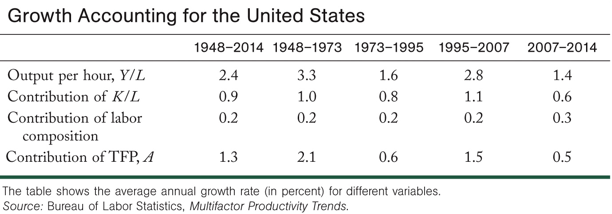
\includegraphics[scale=.55]{growth_accounting}
\end{figure}
\end{frame}


\section{Inflation}

\begin{frame}
\frametitle{\: \: \: Introduction}
\toplinesmall
\begin{itemize}
\item Inflation rate is defined as the rate of change of prices
\begin{eqnarray*}
\pi_{t+1}=\frac{P_{t+1}-P_t}{P_t}
\end{eqnarray*}
\item Inflation in the Canadian economy:
\end{itemize}
\begin{figure}
\centering
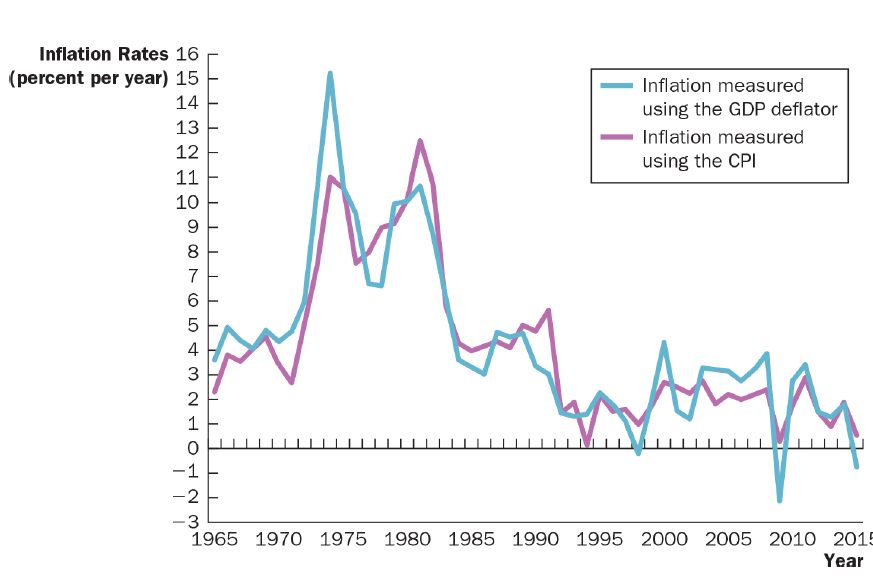
\includegraphics[scale=.4]{inflation_Canada}
\end{figure}
\end{frame}

\begin{frame}
\frametitle{\: \: \: Introduction}
\toplinesmall
\begin{figure}
\centering
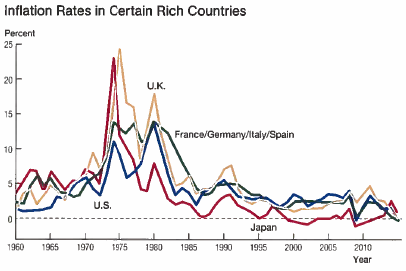
\includegraphics[scale=1]{inflation}
\end{figure}
\end{frame}

\begin{frame}
\frametitle{\: \: \: Introduction}
\toplinesmall
\begin{figure}
\centering
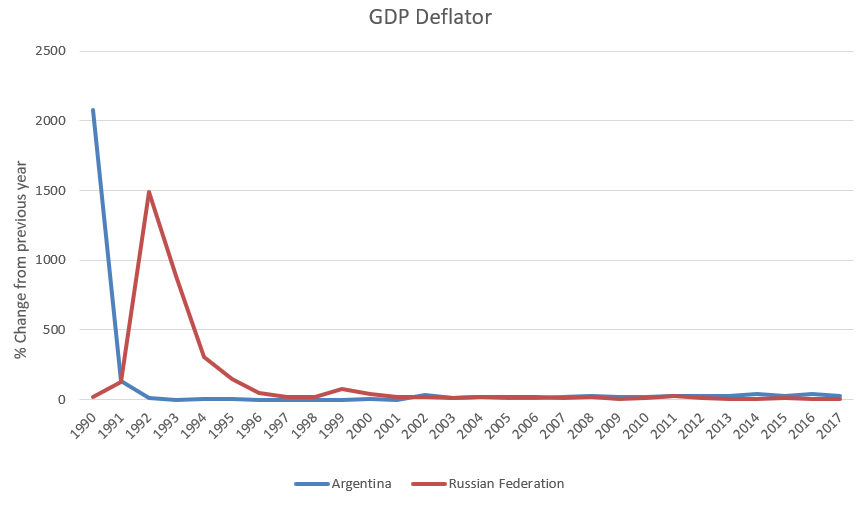
\includegraphics[scale=.6]{hyperinflation1}
\end{figure}
\end{frame}



\begin{frame}
\frametitle{\: \: \: The Quantity Theory of Money}
\toplinexlarge
\begin{itemize}
\item The central component of the quantity theory of money is the quantity equation, which connects nominal GDP with the effective amount of liquidity in circulation:
\begin{eqnarray*}
M_t \: V_t=P_t \: Y_t
\end{eqnarray*}
\begin{itemize}
\item $M_t$=Money Supply
\vspace{.11in}
\item $V_t$=Velocity (the rate at which money changes hands)
\vspace{.11in}
\item $P_t$=Price level
\vspace{.11in}
\item $Y_t$=Real GDP
\end{itemize}
\vspace{.11in}
\item Effective money supply is equal to money demand
\end{itemize}
\end{frame}

\begin{frame}
\frametitle{\: \: \: Prices and Inflation in the Quantity Theory}
\toplinexlarge
\begin{itemize}
\item Classical Dichotomy: real and nominal sides of the economy are separate (money is \textbf{neutral} in the long run).
\vspace{.11in}
\item Prices in the quantity theory of money are given by:
\begin{eqnarray*}
P_t=\frac{M_t \overline{V}}{Y_t}
\end{eqnarray*}
\begin{itemize}
\item Prices are given by how many goods the effective supply of money is chasing.
\end{itemize}
\vspace{.11in}
\item Inflation is given by the following equation:
\begin{eqnarray*}
\Pi=g_M-g_Y
\end{eqnarray*}
\begin{itemize}
\item If the classical dichotomy holds, we should observe that, on average and over the long-run, high inflation correlates with high levels of money supply growth.
\end{itemize}
\end{itemize}
\end{frame}

\begin{frame}
\frametitle{\: \: \: Inflation in the Quantity Theory}
\toplinelarge
\begin{figure}
\centering
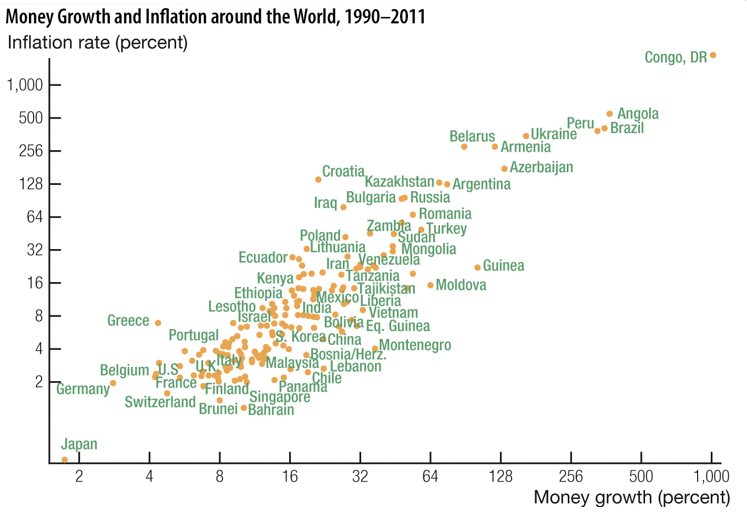
\includegraphics[scale=.5]{money_growth_inflation}
\end{figure}
\end{frame}

\begin{frame}
\frametitle{\: \: \: Risk of Inflation}
\toplinelarge
\begin{itemize}
\item As we will see in the short-run analysis, monetary policy is an important tool to fight recessions (such as the COVID recession)
\vspace{.11in}
\item A risk with loose monetary policy is the risk of increasing the inflation rate over the long-run 
\begin{itemize}
\vspace{.11in}
\item Costs associated with large levels of inflation are well understood.
\vspace{.11in}
\item Large debate over whether this risk has been overblown by economists in recent times (MMT)
\end{itemize}
\end{itemize}
\end{frame}



\begin{frame}
\frametitle{\: \: \: Fisher Equation}
\toplinemedium
\begin{itemize}
\item The Fisher Equation allows us to convert nominal returns on investment into real returns:
\begin{eqnarray*}
i=R+\Pi \Rightarrow R=i-\Pi
\end{eqnarray*}
\begin{itemize}
\item i: nominal interest rate
\item R: real interest rate
\item $\Pi$: inflation rate
\end{itemize}
\vspace{.11in}
\item $R$ depends on the $MPK$, which is usually stable in the short-run
\begin{itemize}
\vspace{.11in}
\item Therefore, the nominal interest rate is usually high when inflation is high
\end{itemize}
\end{itemize}
\end{frame}

\begin{frame}
\frametitle{\: \: \: Fisher Equation}
\toplinemedium
\begin{figure}
\centering
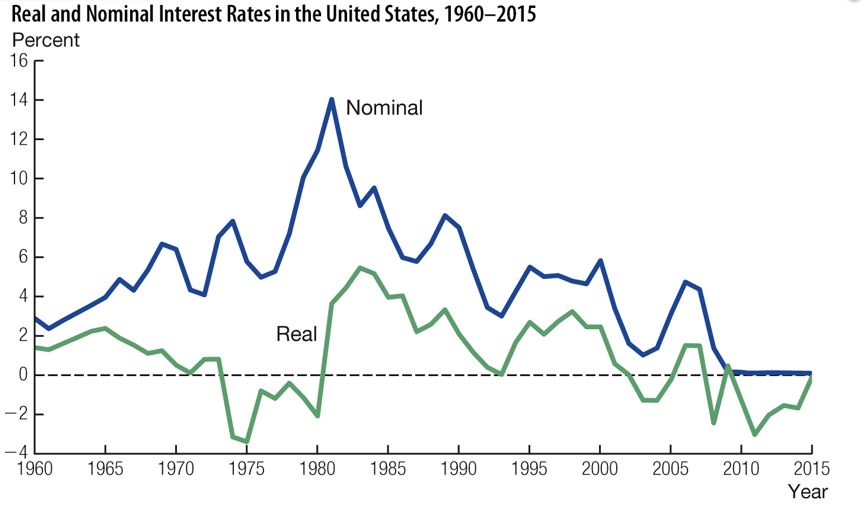
\includegraphics[scale=.5]{nominal_real_interest_rates}
\end{figure}
\end{frame}



\section{Short-Run Macroeconomics}


\begin{frame}
\frametitle{\: \: \: Short-Run Macroeconomics}
\toplinelarge
\begin{itemize}
\item The long-run model is a guide to how the economy behaves on average
\begin{itemize}
\vspace{.11in}
\item Determines potential output and long-run inflation
\end{itemize}
\vspace{.11in}
\item Potential output
\begin{itemize}
\vspace{.11in}
\item Amount of production if all inputs were utilized at their long-run sustainable levels
\end{itemize}
\vspace{.11in}
\item At any given time, the economy is unlikely to exactly equal the long-run average
\vspace{.11in}
\item The short-run model:
\begin{itemize}
\vspace{.11in}
\item Determines current output and current inflation
\end{itemize}
\end{itemize}
\end{frame}

\begin{frame}
\frametitle{\: \: \: Short-Run Macroeconomics}
\toplinelarge
\begin{itemize}
\item Actual output is equal to the long-run trend plus short-run fluctuations:
\begin{eqnarray*}
\underbrace{\text{actual output}}_{Y_t}=\underbrace{\text{long-run trend}}_{\overline{Y}_t}+\underbrace{\text{short-run fluctuations}}_{\text{function of  }\widetilde{Y}_t}
\end{eqnarray*}
\begin{itemize}
\vspace{.11in}
\item Long-run trend: potential ouptut
\vspace{.11in}
\item Short-run fluctuations: deviations from $\overline{Y_t}$
\end{itemize}
\end{itemize}
\end{frame}

\begin{frame}
\frametitle{\: \: \: Short-Run Macroeconomics}
\toplinelarge
\begin{itemize}
\item ``De-trended output'' or short-run output:
\begin{itemize}
\vspace{.11in}
\item The difference in actual and potential output, expressed as a percentage of potential output
\end{itemize}
\begin{eqnarray*}
\widetilde{Y}_t=\frac{Y_t-\overline{Y}_t}{\overline{Y}_t}
\end{eqnarray*}
\end{itemize}
\end{frame}



\begin{frame}
\frametitle{\: \: \: Short-Run Macroeconomics}
\toplinelarge
\begin{columns}
\begin{column}{0.5\linewidth}
\centering
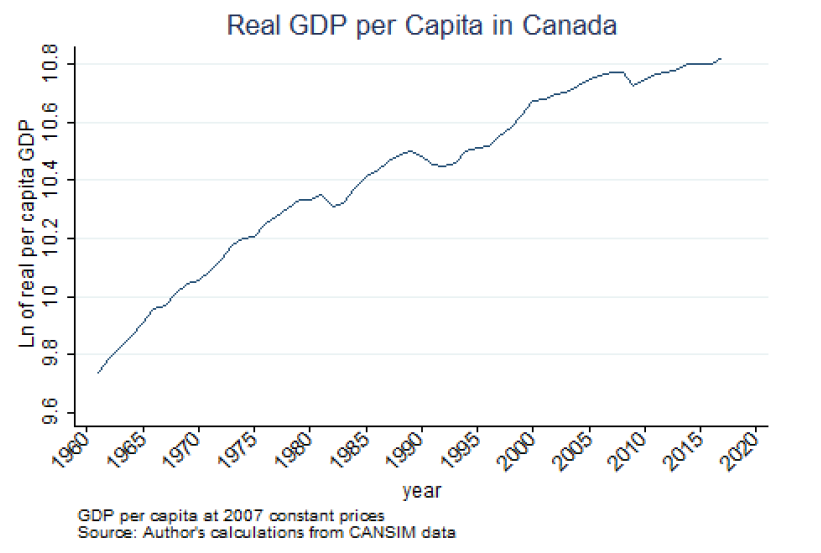
\includegraphics[scale=.25]{GDP_Canada}
\end{column}
\begin{column}{0.5\linewidth}
\centering
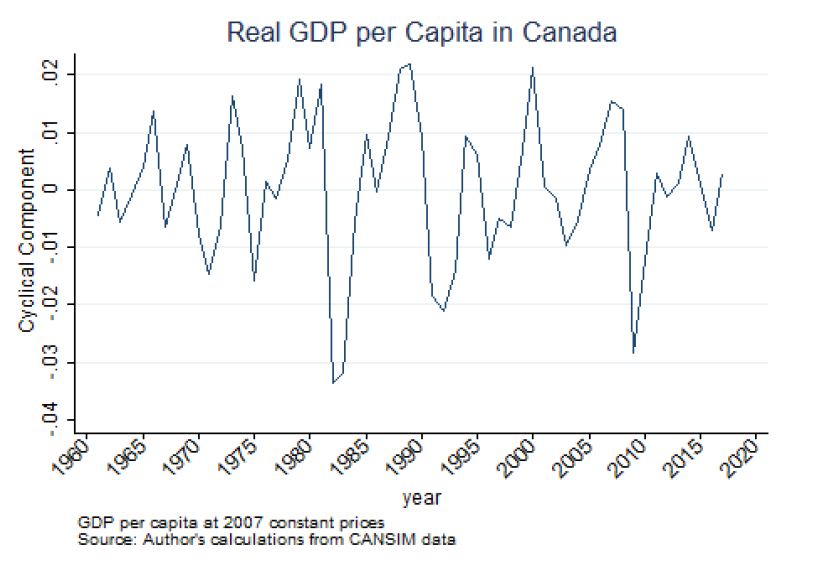
\includegraphics[scale=.25]{SR_GDP_Canada}
\end{column}
\end{columns}
\end{frame}

\begin{frame}
\frametitle{\: \: \: Economics Fluctuations and Unemployment}
\toplinexlarge
\begin{columns}
\begin{column}{0.5\linewidth}
\centering
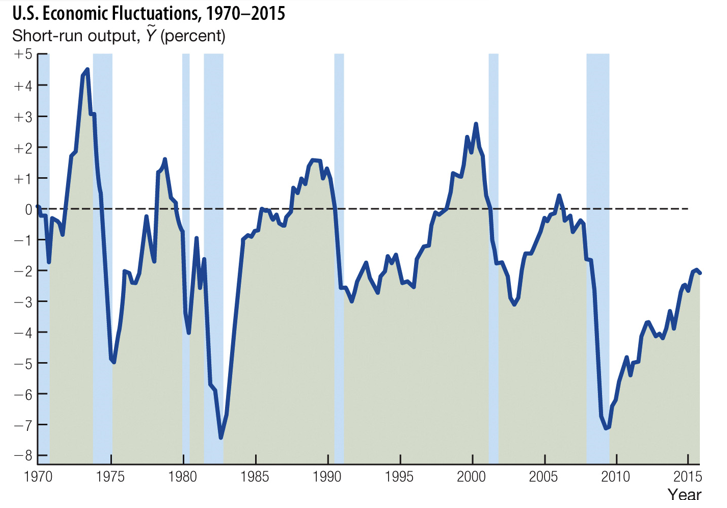
\includegraphics[scale=.3]{US_econ_fluctuations}
\end{column}
\begin{column}{0.5\linewidth}
\centering
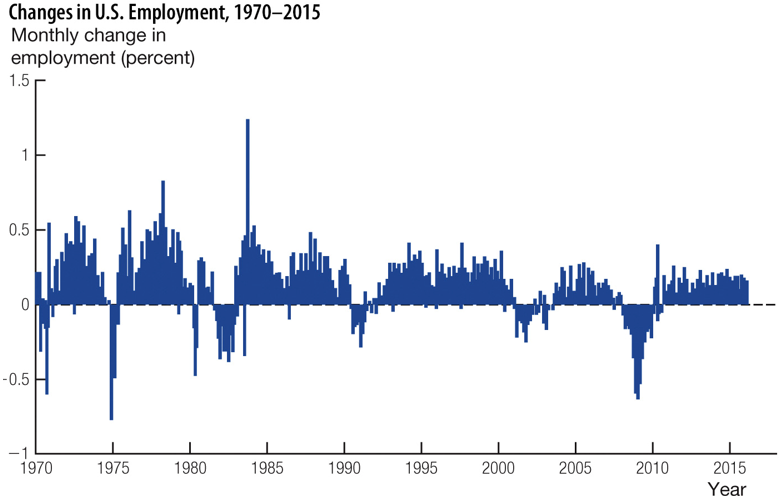
\includegraphics[scale=.3]{US_unemployment}
\end{column}
\end{columns}
\begin{itemize}
\item Recessions are very costly: 
\begin{itemize}
\vspace{.11in}
\item E.g. during a typical recessions GDP per households is around $\$12,000$ below potential output
\vspace{.11in}
\item Unemployment has long-run negative effects on the population.
\end{itemize}
\end{itemize}
\end{frame}




\begin{frame}
\frametitle{\: \: \: Inflation in the Short Run}
\toplinemedium
\begin{columns}
\begin{column}{0.6\linewidth}
\centering
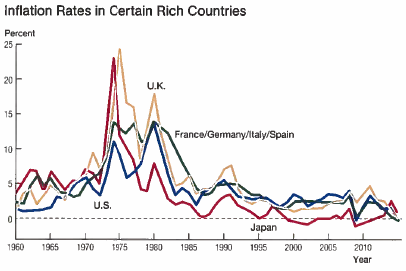
\includegraphics[scale=.8]{inflation}
\end{column}
\begin{column}{0.4\linewidth}
\begin{itemize}
\item Inflation increases during economic booms
\vspace{.11in}
\item Inflation decreases during recessions
\end{itemize}
\end{column}
\end{columns}
\end{frame}

\begin{frame}
\frametitle{\: \: \: Output-Inflation Trade-off}
\toplinelarge
\begin{itemize}
\item The Phillips Curve denotes the output-inflation trade-off:
\end{itemize}
\vspace{.13in}
\centering
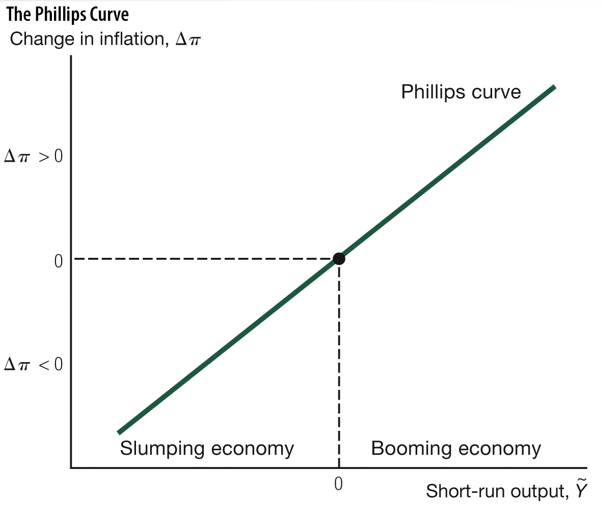
\includegraphics[scale=.5]{phillips_curve}
\end{frame}

\begin{frame}
\frametitle{\: \: \: Phillips Curve in the US}
\toplinelarge
\centering
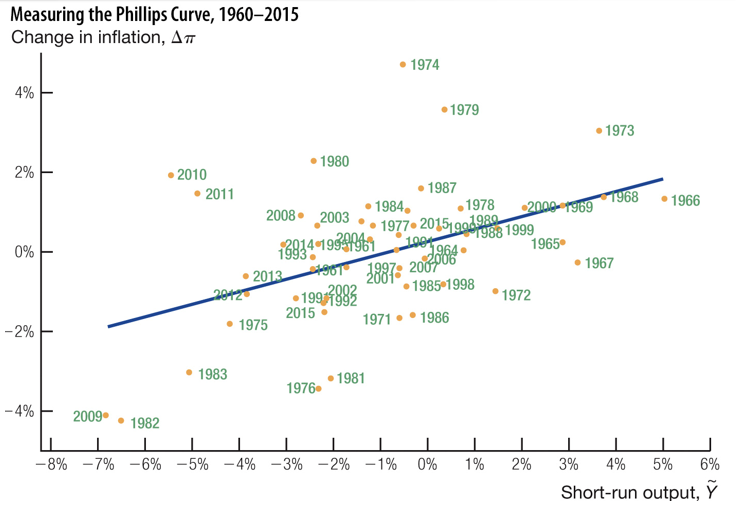
\includegraphics[scale=.5]{US_phillips}
\end{frame}


\begin{frame}
\frametitle{\: \: \: The Basis of the Short-Run Model}
\toplinelarge
\begin{itemize}
\item The economy is constantly being hit by shocks that cause fluctuations in economic activity
\begin{itemize}
\vspace{.11in}
\item Positive shocks increase economic activity beyond its natural rate, which results inflation.
\vspace{.11in}
\item Negative shocks decrease economic activity below its natural rate, which results in recessions.
\end{itemize}
\vspace{.11in}
\item Government through fiscal and monetary policy attempts to neutralize the effects of the shocks.
\vspace{.11in}
\item This creates a constant cycle of boom and bust.
\begin{itemize}
\vspace{.11in}
\item  The duration and severity depends on the shock and government's reaction to the shock.
\end{itemize} 
\end{itemize}
\end{frame}

\begin{frame}
\frametitle{\: \: \: Economic Activity and Unemployment}
\toplinelarge
\begin{itemize}
\item The Short-Run Model analyzes fluctuations in output and not in unemployment
\vspace{.11in}
\item There is a direct connection between unemployment and output, known as Okun's Law:
\begin{eqnarray*}
u-\overline{u}=-\frac{1}{2} \: \: \: \widetilde{Y}
\end{eqnarray*}
\begin{itemize}
\item $u$: current rate of unemployment 
\vspace{.11in}
\item $\overline{u}$: natural rate of unemployment
\vspace{.11in}
\item $\widetilde{Y}$: short-run output
\end{itemize}
\end{itemize}
\end{frame}

\begin{frame}
\frametitle{\: \: \: Okun's Law in the US}
\toplinemedium
\centering
\includegraphics[scale=.5]{okun_law}
\end{frame}

\begin{frame}
\frametitle{\: \: \: Preview of the Short-Run Model}
\toplinelarge
In the remainder of the semester:
\begin{enumerate}
\item We will carefully derive the IS-MP model and study the effects of shocks and government stabilization policy in this framework.
\vspace{.11in}
\item Afterward, we will study the connection between the IS-MP model and the Phillips curve.
\vspace{.11in}
\item Finally, we will put all the parts together and derive a model of the short-run economy, AS-AD, that simulates the periods of boom and bust that characterize modern economies.
\end{enumerate}
\end{frame}



\end{document}